\documentclass[t]{beamer}
\usetheme[darktitle]{UniversityOfManchester}

% Document properties
\title{On-SpiNNaker routing table minimisation}
\author{Andrew Mundy}

% Switch out the fonts
\usepackage{sourcesanspro}
\usepackage{sourcecodepro}

\begin{document}
\maketitle

\begin{frame}{Benchmarks}
  
\end{frame}

\begin{frame}[plain]{}
  \begin{center}
    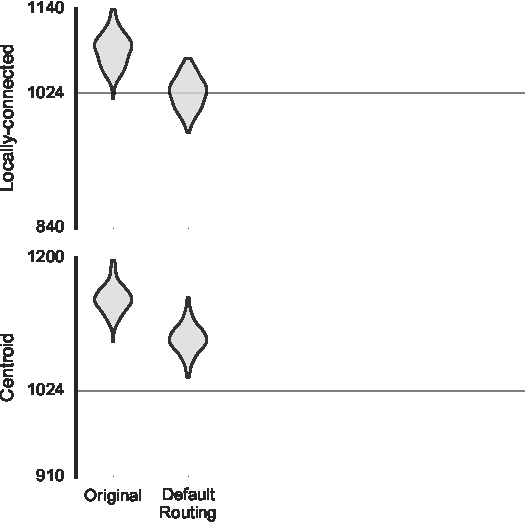
\includegraphics[page=1]{experiments/presentation_plots}
  \end{center}
\end{frame}

\begin{frame}{Minimisation with Espresso}  % Explanation
  
\end{frame}

\begin{frame}[plain]{}
  \begin{center}
    \includegraphics[page=2]{experiments/presentation_plots}
  \end{center}
\end{frame}

\begin{frame}{Order-exploiting minimisation}  % With Espresso, explanation
  
\end{frame}

\begin{frame}[plain]{}
  \begin{center}
    \includegraphics[page=3]{experiments/presentation_plots}
  \end{center}
\end{frame}

\begin{frame}{On-chip routing table minimisation}  % Why?
  % Timing results from Espresso, assume naive scaling
\end{frame}

\begin{frame}[plain]{}
  \begin{center}
    \includegraphics[page=4]{experiments/presentation_plots}
  \end{center}
\end{frame}

\begin{frame}{Ordered-Covering}

\end{frame}

\begin{frame}{\emph{Up-check} rule}
  \begin{center}
    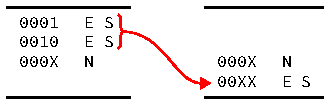
\includegraphics{figures/rule2a_example}
  \end{center}
\end{frame}

\begin{frame}{\emph{Down-check} rule}
  \begin{center}
    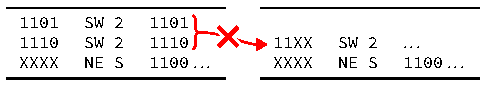
\includegraphics{figures/rule2b_example}
  \end{center}
\end{frame}

\begin{frame}{Resolving the \emph{up-check}}
  \includegraphics<1>{figures/upcheck_resolve_example_1}
  \includegraphics<2>{figures/upcheck_resolve_example_2}
\end{frame}

\begin{frame}{Resolving the \emph{down-check}}
  \begin{center}
    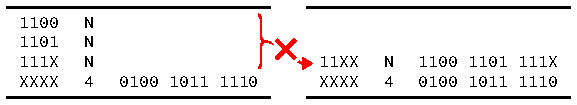
\includegraphics{figures/downcheck_resolve_example_1}
  \end{center}
\end{frame}

\begin{frame}[plain]{}
  \begin{center}
    \includegraphics[page=5]{experiments/presentation_plots}
  \end{center}
\end{frame}

\begin{frame}{On-chip memory usage}
  
\end{frame}

\begin{frame}{Timing}
  
\end{frame}

\begin{darkframes}
  \begin{frame}{}
    \vfill
    \begin{center}
      {\huge Thank You}\\\vskip\baselineskip
      {\Large Any questions?}
    \end{center}
    \vfill
  \end{frame}
\end{darkframes}
\end{document}
